\documentclass[11pt]{article}
\usepackage[margin=1in]{geometry}
\usepackage[T1]{fontenc}
\usepackage{lmodern,microtype}
\usepackage{amsmath,amssymb,amsthm,mathtools}
\usepackage{booktabs,array,enumitem,graphicx,xcolor}
\usepackage{hyperref}
\hypersetup{colorlinks=true,linkcolor=blue!45!black,citecolor=blue!45!black,urlcolor=blue!45!black,pdftitle={Exact laws and hidden dependence in arbitrary symplectic compressions}}
\usepackage{fancyhdr}
\pagestyle{fancy}\fancyhf{}
\fancyhead[L]{\small Exact symplectic compression laws}
\fancyhead[R]{\small Research note}
\fancyfoot[C]{\thepage}
\setlength{\headheight}{14pt}
\setlength{\emergencystretch}{2em}
\numberwithin{equation}{section}
\newtheorem{theorem}{Theorem}[section]
\newtheorem{proposition}[theorem]{Proposition}
\newtheorem{lemma}[theorem]{Lemma}
\newtheorem{corollary}[theorem]{Corollary}
\theoremstyle{definition}
\newtheorem{definition}[theorem]{Definition}
\newtheorem{example}[theorem]{Example}
\theoremstyle{remark}
\newtheorem{remark}[theorem]{Remark}
\newcommand{\F}{\mathbb F}
\newcommand{\N}{\mathbb N}
\newcommand{\Prob}{\mathbb P}
\newcommand{\E}{\mathbb E}
\newcommand{\TV}{d_{\mathrm{TV}}}
\newcommand{\Mat}{\operatorname{Mat}}
\newcommand{\Alt}{\operatorname{Alt}}
\newcommand{\Sp}{\operatorname{Sp}}
\newcommand{\GL}{\operatorname{GL}}
\newcommand{\rank}{\operatorname{rank}}
\newcommand{\rad}{\operatorname{rad}}
\newcommand{\im}{\operatorname{im}}
\newcommand{\tr}{\mathsf T}
\newcommand{\qbin}[2]{\genfrac{[}{]}{0pt}{}{#1}{#2}_{q}}
\newcommand{\abs}[1]{\lvert#1\rvert}
\newcommand{\set}[1]{\{#1\}}
\newcommand{\code}[1]{\nolinkurl{#1}}
\newcommand{\Binf}{B_\infty(q)}
\newcommand{\Oinf}{O_\infty(q)}
\newcommand{\sourcecommit}{\texttt{72fead102f663d5c7a407964a13dc0cf9d977207}}
\newcommand{\articlecommit}{\texttt{fc9889c80312959aee9893ab21bfc9e741719e88}}

\title{\textbf{Exact laws and hidden dependence\\in arbitrary symplectic compressions}\\[0.6em]
\large A solution to the general-compression question in the supplied GRH article}
\author{Research note prepared for Vladimir Reshetnikov}
\date{November 26, 2026}

\begin{document}
\maketitle
\begin{abstract}
The supplied article on transfers from the Dirichlet-GRH development asks for the law of a finite symplectic matrix compressed between two arbitrary subspaces, beyond its isotropic and Lagrangian cases. We give every point probability, including all degeneracies and characteristic two. The likelihood depends on three integers obtained from the joint alternating Gram matrix. The same calculation gives an exact support criterion, the smallest ambient symplectic dimension realizing prescribed pairings, and the conditional intersection law.

Two quantitative consequences go beyond the enumeration. For fixed block dimensions, the distance to an independent-entry matrix has an explicit positive leading coefficient times $q^{-2N}$, where $2N$ is the ambient dimension. At the opposite, complementary-dimension boundary, with both subspaces nondegenerate, a singularity test of a residual alternating form is exactly optimal. Along increasingly tall blocks with both dimensions growing, every rank-only test has vanishing advantage, but the full-matrix total-variation distance tends to an explicit positive constant, approximately $0.1306343467$ over $\F_2$.

All new theorems in this note are unconditional. They extend a finite-linear-algebra component of the supplied research program; they do not assert a further Riemann hypothesis. Classical form-representation counts are credited, and global priority for the resulting formulas is not claimed established. Complete proofs and independent exhaustive finite checks are supplied.
\end{abstract}
\clearpage
\tableofcontents
\clearpage

\section{What is extracted from the two repositories}
\label{sec:sources}

\subsection{The exact upstream theorem and mechanism}
The inspected version of \code{lsernau/grh-lean} is commit
\begin{center}\sourcecommit.\end{center}
Its public \code{grh/src/Statements.lean} imports only Mathlib. The five declarations in \code{grh/src/Main.lean} prove Mathlib's \code{RiemannHypothesis}, a statement locating all nontrivial zeta zeros, nonvanishing of Dirichlet $L$-functions in $\Re s>1/2$ away from the pole, and the corresponding critical-strip statements for all Dirichlet characters and for primitive characters \cite{upstream}. Thus the relevant input is \emph{Dirichlet} GRH, including imprimitive characters. It does not state GRH for every Artin or automorphic $L$-function.

The upstream README reports a build without \code{sorry}, axiom dependencies
\code{propext}, \code{Classical.choice}, \code{Quot.sound}, and acceptance of exports by independent checkers. This note inspected the statements and selected proof files; it did not rebuild or replay the complete development. The reported validation is attributed to the upstream project.

The transferable architecture is a comparison of upper and lower bounds for the same integral covolume. Short integral source forms give the upper bound, a second-moment argument supplies enough independent images, and twisted determinants with controlled denominators give the lower bound. After cancellation of the common main term, \code{New.star_inequality} yields
\[
 m\,\mathrm{totalRemainder}\le f a(\log B)^5.
\]
Here $m$ is the number of lifts and the other parameters belong to the source construction. The scale choices turn this into an eventual one-sided estimate for a smoothed prime remainder. The final analytic argument uses a suitable quadratic twist and Landau's positivity argument to exclude zeros. The precise inequalities and assumptions are described in the accompanying source audit and linked to pinned files.

The finite-field compression problem arises in the article's analysis of the spanning and matrix-statistics interface. The present work follows that branch of the transfer program. Its proofs use finite symplectic geometry and probability, so the analytic RH/GRH theorem is not a logical hypothesis below.

\subsection{The exact question answered}
The inspected ProveIt revision is
\begin{center}\articlecommit.\end{center}
The article README describes a merge of 103 reports with 760 results. It explicitly says the merge is not an independent review. In \code{Article/sections/spn.tex}, the question labeled \code{spn:q:symplectic} asks for the law of arbitrary symplectic compressions, when neither compressed subspace need be Lagrangian \cite{article}. The preceding results cover isotropic pairs and a Lagrangian target with an arbitrary source form. They also show that rank tests can miss dependence in that particular Lagrangian setting.

This note answers the exact-law part of that question for \emph{all} subspace types and all dimensions in which the individual spaces embed. It also gives a new nondegenerate, rectangular family with an exact optimal test and a different limiting constant. This is a precise extension of the supplied article, rather than a claim to have discovered rank blindness for the first time.

\subsection{Relation to prior counting theory}
Counts of representations of alternating forms, including prescribed total rank, are classical. Wan \cite{wan} and Wei--Zhang \cite{weizhang} are particularly relevant; the latter also records earlier work of Carlitz, Hodges and Buckhiester. Guo--Li--Wang \cite{guo} study symplectic subspace counts, and De Boeck--Van de Voorde \cite{deboeck} give exact counts with disjointness and nondegeneracy conditions.

We therefore make no novelty claim for the embedding factor in Lemma~\ref{lem:embeddings}, or for elementary Gaussian-binomial enumeration. The useful refinement here is to require \emph{separate injectivity on both coordinate blocks}, then calculate the full cross-Gram likelihood, its exact support, and the two sharp probabilistic regimes. No identical full package was located in the sources inspected. Full text of some older articles was unavailable, so this establishes an extension relative to the supplied article, not a definitive global priority claim. The accompanying literature review records what was checked.

\section{The exact law for arbitrary compressed subspaces}
\label{sec:law}

\subsection{Setup and three observable invariants}
Let $q$ be any prime power. An alternating form over $\F_q$ has a matrix $A$ satisfying $A^\tr=-A$ and zero diagonal; the latter condition is essential in characteristic two. Let $(V,\omega)$ be a nondegenerate alternating space of dimension $2N$. Fix injective linear maps
\[
 X:U=\F_q^a\longrightarrow V,
 \qquad Y_0:W=\F_q^b\longrightarrow V.
\]
In a fixed basis of $V$, let $J$ represent $\omega$, and put
\[
 F=X^\tr JX,\quad H=Y_0^\tr JY_0,\quad
 \rank F=2f,\quad \rank H=2h.
\]
The spaces $\im X$ and $\im Y_0$ can be degenerate and can intersect. Draw $g$ uniformly from the finite group $\Sp(V)$ and observe
\begin{equation}\label{eq:observation}
 \mathcal M=X^\tr JgY_0\in\Mat_{a\times b}(\F_q).
\end{equation}
This includes the usual row-column compression: the nondegenerate pairing identifies a space of row functionals with a subspace of $V$. Let $Z$ denote an independent-entry uniform $a\times b$ matrix.

For a candidate observation $M$, define its joint Gram matrix and invariants by
\begin{align}
 G_M&=\begin{pmatrix}F&M\\-M^\tr&H\end{pmatrix},
 &\rank G_M&=2s,\label{eq:joint}\\
 R&=\rad G_M,&r&=a+b-2s,\notag\\
 u&=\dim(R\cap(U\oplus0)),
 &v&=\dim(R\cap(0\oplus W)),\label{eq:uv}\\
 c&=r-u-v.&&\notag
\end{align}
In particular $c\ge0$. These are readily computed by elimination:
\begin{equation}\label{eq:computeuv}
 u=\dim(\ker F\cap\ker M^\tr),\qquad
 v=\dim(\ker H\cap\ker M).
\end{equation}
Once $a,b,F,H$ are fixed, only the three integers $(s,u,v)$ vary in the probability formula. This is a statement about the likelihood; it need not classify every geometric orbit of pairs.

Write $\qbin nk$ for the Gaussian binomial coefficient, defined to be zero outside $0\le k\le n$, and put
\[
 \gamma_j(q)=\abs{\GL_j(\F_q)}=\prod_{i=0}^{j-1}(q^j-q^i),\qquad \gamma_0(q)=1.
\]
Define
\begin{equation}\label{eq:T}
 T_d(r,u,v)=
 \sum_{j=\max(0,d-c)}^{\min(u,v,d)}
 \qbin uj\qbin vj\gamma_j(q)\qbin c{d-j}
 q^{(d-j)(u+v-j)}.
\end{equation}
An empty sum is zero. Finally, set
\begin{equation}\label{eq:E}
 E_N(k,t)=q^{2Nk-\binom k2}
 \prod_{i=N-k+t+1}^{N}(1-q^{-2i})
 \quad\text{if }0\le2t\le k\text{ and }k-t\le N,
\end{equation}
and $E_N(k,t)=0$ otherwise. Empty products are one. Although written with negative powers, every nonzero $E_N$ is an integer.

\begin{theorem}[Complete arbitrary-compression law]\label{thm:law}
In the setup above, for every $M\in\Mat_{a\times b}(\F_q)$,
\begin{equation}\label{eq:law}
 \boxed{\displaystyle
 \Prob(\mathcal M=M)=
 \frac{\displaystyle\sum_{d=0}^{r-\max(u,v)}
 T_d(r,u,v)E_N(a+b-d,s)}{E_N(a,f)E_N(b,h)}.}
\end{equation}
The denominator is positive. Every summand is nonnegative. The likelihood relative to $Z$ is $q^{ab}$ times \eqref{eq:law}. In particular the three invariants $(s,u,v)$ suffice to evaluate the optimal likelihood test.
\end{theorem}

The formula consists of finite sums of explicit products. It does not enumerate $\Sp(V)$ or require a classification of its double cosets. Its number of summands and displayed product factors is polynomial in $a+b$; computing the integer powers and evaluating large integers has its own bit complexity.

\subsection{Embedding a possibly degenerate alternating space}
\begin{lemma}[Classical embedding count]\label{lem:embeddings}
The number of injective isometries from a specified alternating $k$-space of rank $2t$ to a nondegenerate alternating $2N$-space is $E_N(k,t)$. Such an embedding exists if and only if $k-t\le N$. The symplectic group is transitive on these embeddings.
\end{lemma}
\begin{proof}
Split the domain into a nondegenerate $2t$-space and its radical of dimension $\ell=k-2t$. Choose the images of its $t$ symplectic basis pairs in order. At the $i$th step the remaining nondegenerate space has dimension $2N-2i$. The first vector has $q^{2N-2i}-1$ choices; the vector with prescribed pairing one has $q^{2N-2i-1}$ choices. Their span is nondegenerate, so pass to its orthogonal complement.

The images of the radical basis must then form an independent isotropic $\ell$-frame in dimension $2(N-t)$. After $i$ radical vectors, the next lies in their common orthogonal complement but outside their span. There are
\[
 q^{2(N-t)-i}-q^i
\]
choices. Consequently the count is
\begin{equation}\label{eq:integerE}
 \prod_{i=0}^{t-1}(q^{2N-2i}-1)q^{2N-2i-1}
 \prod_{i=0}^{\ell-1}(q^{2(N-t)-i}-q^i).
\end{equation}
It is positive exactly when $\ell\le N-t$, equivalently $k-t\le N$. Extracting powers of $q$ combines the remaining factors into \eqref{eq:E}.

For transitivity, an isometry between the two image subspaces extends to the ambient space. Here is the usual alternating-form version of Witt extension. Match the nondegenerate summands first and pass to their orthogonal complements. Complete the corresponding radical bases to hyperbolic pairs by choosing dual partners. Successive additions of radical vectors to the partners remove their mutual pairings, using only triangular adjustments, with no division by two. Complete both resulting nondegenerate spans to symplectic bases. The map between these bases is the required ambient isometry. This also covers characteristic two and degenerate initial subspaces.
\end{proof}

\subsection{Counting kernels that preserve injectivity on both blocks}
\begin{lemma}[Two forbidden coordinate subspaces]\label{lem:kernels}
Let $A,B$ be disjoint subspaces of an $r$-space $R$, of dimensions $u,v$. Then $T_d(r,u,v)$ counts the $d$-subspaces $D\le R$ satisfying $D\cap A=D\cap B=0$. Moreover
\begin{equation}\label{eq:Tpositive}
 T_d(r,u,v)>0\quad\Longleftrightarrow\quad
 0\le d\le r-\max(u,v).
\end{equation}
\end{lemma}
\begin{proof}
Choose a splitting $R=A\oplus B\oplus C$ with $\dim C=c$. For such a $D$, let
$j=\dim(D\cap(A\oplus B))$. Since this intersection meets neither $A$ nor $B$, both coordinate projections are injective on it. It is therefore the graph of an isomorphism between a $j$-subspace of $A$ and a $j$-subspace of $B$. There are
\[
 \qbin uj\qbin vj\gamma_j(q)
\]
choices. The projection of $D$ to $C$ is a $(d-j)$-subspace, with $\qbin c{d-j}$ choices. After these choices, $D$ is determined by a linear map from that projection into
$(A\oplus B)/(D\cap(A\oplus B))$, a space of dimension $u+v-j$. This gives the power of $q$ in \eqref{eq:T}.

The allowable dimensions satisfy $j\le\min(u,v)$ and $d-j\le c$. All dimensions from zero through $c+\min(u,v)$ are attained by a graph and a subspace of $C$. Since $c+\min(u,v)=r-\max(u,v)$, this proves \eqref{eq:Tpositive}.
\end{proof}

\subsection{Proof of the complete law}
\begin{proof}[Proof of Theorem~\ref{thm:law}]
By Lemma~\ref{lem:embeddings}, $Y=gY_0$ is uniform among the $E_N(b,h)$ injective maps with Gram matrix $H$. Concatenate a pair of injective maps as
\[
 Z_{X',Y'}:U\oplus W\longrightarrow V,\qquad (x,y)\longmapsto X'x+Y'y.
\]
If its Gram matrix is $G_M$, then its kernel $D$ is contained in $R=\rad G_M$. Separate injectivity is exactly the condition that $D$ meet neither coordinate summand. Within $R$, these two intersections are $A=R\cap U$ and $B=R\cap W$. Thus there are $T_d(r,u,v)$ possible kernels of dimension $d$.

For each fixed such kernel, the form descends to $(U\oplus W)/D$, whose dimension is $a+b-d$ and whose form rank is still $2s$. An injective isometry of this quotient into $V$ determines, and is determined by, a concatenated map with exactly that kernel. Lemma~\ref{lem:embeddings} counts these maps as $E_N(a+b-d,s)$.

So far the first frame $X'$ has been allowed to vary. Every one of its $E_N(a,f)$ possible values has the same number of extensions: an ambient symplectic map taking one first frame to another gives a bijection of extensions and preserves the domain kernel. Divide by $E_N(a,f)$ to fix the given $X$. Finally divide by the $E_N(b,h)$ equally likely second frames. This proves \eqref{eq:law}.
\end{proof}

\section{Exact support, minimal ambient dimension and intersections}
\label{sec:support}

\begin{theorem}[Support and optimal symplectic completion]\label{thm:support}
A candidate $M$ occurs with positive probability if and only if
\begin{equation}\label{eq:support}
 \boxed{s+\max(u,v)\le N.}
\end{equation}
More generally, given any alternating $F,H$ and any cross-pairing matrix $M$, without specifying an ambient space in advance, the least dimension of a nondegenerate alternating space realizing these data by two injective maps is
\begin{equation}\label{eq:minimal}
 \boxed{2\bigl(s+\max(u,v)\bigr).}
\end{equation}
\end{theorem}
\begin{proof}
The quotient corresponding to a $d$-dimensional kernel embeds if and only if
\[
 a+b-d-s\le N,
 \quad\text{or}\quad d\ge a+b-s-N.
\]
Lemma~\ref{lem:kernels} allows exactly $0\le d\le r-\max(u,v)$. These intervals meet if and only if
\[
 a+b-s-N\le a+b-2s-\max(u,v),
\]
which is \eqref{eq:support}.

For the second assertion take a maximal permitted kernel of dimension $r-\max(u,v)$. The quotient has dimension $2s+\max(u,v)$ and radical dimension $\max(u,v)$. Pairing its radical with new dual vectors completes it to a symplectic space of dimension $2(s+\max(u,v))$. The first inequality proves that a smaller dimension is impossible. The quotient map remains injective on both original summands, giving a realization, not merely a numerical necessary condition.
\end{proof}

\begin{corollary}[Conditional intersection geometry]\label{cor:intersection}
For a supported $M$, all integers in the interval
\begin{equation}\label{eq:intersectionrange}
 \max(0,a+b-s-N)\le d\le r-\max(u,v)
\end{equation}
occur as $\dim(\im X\cap\im(gY_0))$. Conditional on $\mathcal M=M$, their probabilities are
\begin{equation}\label{eq:posterior}
 \frac{T_d(r,u,v)E_N(a+b-d,s)}
 {\sum_eT_e(r,u,v)E_N(a+b-e,s)}.
\end{equation}
Given $d$, the concatenated kernel is uniform among the $T_d$ permitted subspaces.
\end{corollary}
\begin{proof}
For separately injective $X,Y$, the map $(x,y)\mapsto Xx=-Yy$ identifies the concatenated kernel with the intersection of their image subspaces. The count in the proof of Theorem~\ref{thm:law} gives \eqref{eq:posterior}; both factors are positive exactly on \eqref{eq:intersectionrange} and do not depend on the particular kernel of fixed dimension.
\end{proof}

\begin{example}[Equal ordinary rank, different feasibility]\label{ex:support}
Over $\F_3$, let $a=b=2$, $F=H=J_1=\left(\begin{smallmatrix}0&1\\-1&0\end{smallmatrix}\right)$. Compare $M_1=I_2$ and $M_2=\operatorname{diag}(1,2)$; both have rank two. For a $2\times2$ matrix, $M^\tr J_1M=(\det M)J_1$. The Schur complement of $F$ in $G_M$ is therefore $(1-\det M)J_1$. Hence $G_{M_1}$ has rank two and $G_{M_2}$ has rank four, while $u=v=0$ in both cases. The first candidate can be realized in ambient dimension two; the second needs dimension four. Ordinary matrix rank does not decide even the support of a general compression law.
\end{example}

\section{An exact rational likelihood and the sharp fixed-size rate}
\label{sec:fixed}
Fix $q,a,b,F,H$ while $N$ increases. The individual frames exist for $N\ge\max(a-f,b-h)$. Put $k=a+b$ and
\[
 t=q^{-2N},\qquad P_\ell(t)=\prod_{i=0}^{\ell-1}(1-q^{2i}t),\qquad
 S_\ell=\sum_{i=0}^{\ell-1}q^{2i}=\frac{q^{2\ell}-1}{q^2-1}.
\]
The conventions $P_0=1$, $S_0=0$ apply.

\begin{proposition}[Exact rational expression]\label{prop:rational}
For every admissible $N$, the likelihood $L_N(M)=q^{ab}\Prob(\mathcal M=M)$ equals
\begin{equation}\label{eq:rational}
 L_N(M)=
 \frac{\displaystyle\sum_{d=0}^{r-\max(u,v)}
 T_d(r,u,v)q^{dk-d(d+1)/2}t^dP_{k-d-s}(t)}
 {P_{a-f}(t)P_{b-h}(t)}.
\end{equation}
\end{proposition}
\begin{proof}
Substitute \eqref{eq:E} in \eqref{eq:law}. The power of $q$ in its $d$th term, including the uniform normalization, is
\[
 ab+2N(k-d)-\binom{k-d}{2}-2Na+\binom a2-2Nb+\binom b2
 =-2Nd+dk-\frac{d(d+1)}2.
\]
The product factor is $P_{k-d-s}(t)$. If this quotient space cannot embed, $k-d-s>N$ and the product contains $1-q^{2N}t=0$, so the expression still gives zero. The denominator is nonzero for the stipulated admissible $N$.
\end{proof}

For probability laws on a finite set, write
$\TV(P,Q)=\tfrac12\sum_x\abs{P(x)-Q(x)}$. It is also the maximum difference of event probabilities.

\begin{theorem}[Explicit first correction and optimal rate]\label{thm:fixed}
For fixed $q,a,b,F,H$, uniformly in $M$,
\begin{equation}\label{eq:firstorder}
 L_N(M)=1+A(M)q^{-2N}+O_{q,a,b}(q^{-4N}),
\end{equation}
where
\begin{equation}\label{eq:A}
 A(M)=S_{a-f}+S_{b-h}-S_{k-s}
 +q^{k-1}\frac{q^r-q^u-q^v+1}{q-1}.
\end{equation}
Consequently
\begin{align}
 \TV(\mathcal M,Z)&=C_{q,F,H}\,q^{-2N}+O_{q,a,b}(q^{-4N}),\label{eq:fixedTV}\\
 C_{q,F,H}&=\frac{1}{2q^{ab}}\sum_{M\in\Mat_{a\times b}(\F_q)}\abs{A(M)}.\label{eq:C}
\end{align}
If $a,b\ge1$, then
\begin{equation}\label{eq:positiveC}
 C_{q,F,H}\ge\frac{q-1}{q}>0.
\end{equation}
Thus every nonempty fixed-size compression has the exact order of convergence $\Theta(q^{-2N})$.
\end{theorem}
\begin{proof}
There is one zero-dimensional kernel. The number of permitted lines is all lines in $R$, minus those in each of its disjoint coordinate radicals:
\[
 T_0=1,\qquad T_1=\frac{q^r-q^u-q^v+1}{q-1}.
\]
In \eqref{eq:rational}, use $P_\ell(t)=1-S_\ell t+O(t^2)$; terms with $d\ge2$ are $O(t^2)$. This gives \eqref{eq:A}. There are finitely many possible matrices and forms for fixed $q,a,b$, so the error can be chosen uniformly. Summing \eqref{eq:firstorder}, using $\bigl|\abs{x+e}-\abs x\bigr|\le\abs e$, gives \eqref{eq:fixedTV}.

For positivity, take any one matrix entry. It is the pairing of a fixed nonzero vector $x$ with a vector uniform on $V\setminus\set0$. Thus
\[
 \Prob(\mathcal M_{ij}=0)=\frac{q^{2N-1}-1}{q^{2N}-1},
 \qquad
 \frac1q-\Prob(\mathcal M_{ij}=0)=\frac{q-1}{q(q^{2N}-1)}.
\]
Total variation cannot increase when only one coordinate is observed. Multiply this lower bound by $q^{2N}$ and let $N\to\infty$ in \eqref{eq:fixedTV} to obtain \eqref{eq:positiveC}.
\end{proof}

For $a=b=1$, $F=H=0$, one has $A(0)=1-q$ and $A(M)=1$ for $M\ne0$. The coefficient $(q-1)/q$ is attained, and the exact distance is $(q-1)/(q(q^{2N}-1))$. The theorem is a fixed-dimension result; its implicit constants are not uniform when the block dimensions grow with $N$. The next section treats a different regime explicitly.

\section{Both subspaces nondegenerate: an exact optimal test}
\label{sec:boundary}
Assume now that $a,b$ are positive even integers, both $F$ and $H$ are nonsingular, and the ambient dimension is their sum:
\begin{equation}\label{eq:boundarysetup}
 2N=a+b.
\end{equation}
Neither subspace is Lagrangian. Put $h=b/2$ and
\begin{align}
 K(M)&=H+M^\tr F^{-1}M,\label{eq:K}\\
 B_j&=\prod_{i=1}^j(1-q^{-2i}),\quad B_0=1,
 &C_{a,b}&=\prod_{i=a/2+1}^{(a+b)/2}(1-q^{-2i}).\label{eq:BC}
\end{align}
The matrix $K(M)$ is alternating in every characteristic. Since $b$ is even, write its corank as $2\ell$.

\begin{theorem}[Likelihood and the optimal residual test]\label{thm:boundary}
For every $M$, its likelihood relative to the independent-entry model is
\begin{equation}\label{eq:boundarylikelihood}
 L(M)=\frac{B_h}{C_{a,b}}
 \sum_{d=\ell}^{2\ell}
 \qbin{2\ell}d\frac{q^{-d(d+1)/2}}{B_{d-\ell}}.
\end{equation}
It is strictly less than one when $K(M)$ is nonsingular, and strictly greater than one when $K(M)$ is singular. Therefore the event
\begin{equation}\label{eq:optimaltest}
 \boxed{K(M)\text{ is singular}}
\end{equation}
is an exact optimal distinguishing event. In particular
\begin{equation}\label{eq:boundaryTV}
 \boxed{\displaystyle
 \TV(\mathcal M,Z)=
 \left(1-\frac{B_h}{C_{a,b}}\right)
 \Prob\bigl(K(Z)\text{ is nonsingular}\bigr).}
\end{equation}
\end{theorem}

\subsection{Proof of the likelihood}
\begin{proof}[Proof of \eqref{eq:boundarylikelihood}]
Since $\im X$ is nondegenerate, decompose $V=\im X\oplus(\im X)^\perp$. The second summand has dimension $b=2h$; choose a symplectic basis there with matrix $J_h=\left(\begin{smallmatrix}0&I_h\\-I_h&0\end{smallmatrix}\right)$. The condition $X^\tr JY=M$ uniquely fixes the component of $Y$ in $\im X$ as $XF^{-1}M$. Its Gram matrix is
\[
 (F^{-1}M)^\tr F(F^{-1}M)=-M^\tr F^{-1}M.
\]
Writing the other component as a $b\times b$ matrix $T$, the remaining equation is
\begin{equation}\label{eq:residualgram}
 T^\tr J_hT=K(M).
\end{equation}
The full $Y$ is automatically injective because $Y^\tr JY=H$ is nonsingular.

The kernel of a map satisfying \eqref{eq:residualgram} is a $d$-subspace of $\rad K$, which has dimension $2\ell$. Each such kernel gives an embedding of a $(b-d)$-space of rank $b-2\ell$ into a symplectic $b$-space. The admissible dimensions are $\ell\le d\le2\ell$. Therefore the number of solutions is
\begin{equation}\label{eq:residualcount}
 \sum_{d=\ell}^{2\ell}\qbin{2\ell}d E_h(b-d,h-\ell).
\end{equation}
Using \eqref{eq:E} gives
\[
 E_h(b-d,h-\ell)
 =q^{b(b+1)/2-d(d+1)/2}\frac{B_h}{B_{d-\ell}}.
\]
The total number of eligible $Y$ is $E_N(b,h)$, and
\[
 q^{-ab}E_N(b,h)=q^{b(b+1)/2}C_{a,b}.
\]
Dividing \eqref{eq:residualcount} by this expression proves the likelihood formula.
\end{proof}

\subsection{Proof that the singularity test is exactly optimal}
\begin{proof}[Proof of the sign assertions and \eqref{eq:boundaryTV}]
If $\ell=0$, the sum is one. Each of the $h$ factors defining $C_{a,b}$ has a larger index than the corresponding factor in $B_h$, since $a>0$. Thus $B_h/C_{a,b}<1$.

Define $\Binf=\prod_{i\ge1}(1-q^{-2i})$. The elementary inequality $\prod_i(1-x_i)\ge1-\sum_ix_i$ gives
\begin{equation}\label{eq:Bbound}
 \Binf\ge1-\frac1{q^2-1}>0.
\end{equation}
For $\ell=1$, the two terms of the sum simplify to
\[
 (q+1)q^{-1}+\frac{q^{-3}}{1-q^{-2}}
 =1+\frac{q}{q^2-1}.
\]
Multiplying by the lower bound in \eqref{eq:Bbound} gives a number strictly greater than one: the difference from one is
\[
 \frac{(q-1)(q^2-1)-q}{(q^2-1)^2}>0\qquad(q\ge2).
\]
Since $B_h/C_{a,b}\ge\Binf$, this proves the required sign when $\ell=1$.

For $\ell\ge2$, just the $d=\ell$ term gives
\[
 L(M)\ge\Binf\qbin{2\ell}\ell q^{-\ell(\ell+1)/2}
 \ge\Binf q^{\ell(\ell-1)/2}>1.
\]
Here $\qbin{2\ell}\ell\ge q^{\ell^2}$, and $q\Binf>1$ follows already from \eqref{eq:Bbound}.

For finite laws, the event where the likelihood exceeds one realizes total variation. All excess mass is on the singular residuals, and all deficient mass on the nonsingular residuals. The likelihood on the latter set is the constant $B_h/C_{a,b}$, proving \eqref{eq:boundaryTV}.
\end{proof}

\begin{example}[A small exact calculation]\label{ex:q3}
Let $q=3$, $a=b=2$, and $F=H=J_1$. Then $K(M)=(1-\det M)J_1$ and
\[
 L(M)=\begin{cases}99/80,&\det M=1,\\9/10,&\det M\ne1.\end{cases}
\]
Exactly $24$ of the $81$ matrices have determinant one. Hence
\[
 \TV(\mathcal M,Z)=\frac{19}{270}.
\]
Matrices of determinants one and two both have full ordinary rank but lie on opposite sides of the likelihood threshold. In this example the distance between the rank laws is only $11/270$.
\end{example}

\begin{corollary}[Persistent dependence for every balanced nondegenerate family]\label{cor:allboundary}
For every positive even $a,b$ with ambient dimension $a+b$,
\begin{equation}\label{eq:uniformlower}
 \TV(\mathcal M,Z)\ge
 \left(1-\frac{B_h}{C_{a,b}}\right)
 \left(1-\frac{q(1-q^{-a})(1-q^{-b})}{q^2-1}\right).
\end{equation}
In particular, whenever $a,b\to\infty$, even if $a=b$,
\[
 \liminf\TV(\mathcal M,Z)\ge
 (1-\Binf)\left(1-\frac{q}{q^2-1}\right)>0.
\]
\end{corollary}
\begin{proof}
For a fixed nonzero domain vector $x$, change coordinates so that $x$ is the first basis vector. Write $z_1,\ldots,z_b$ for the independent uniform columns of $Z$, with the correspondingly changed nonsingular $H$. If $z_1=0$, the equation $K(Z)x=0$ is impossible, because the first column of $H$ is nonzero. If $z_1\ne0$, its pairing with each of the remaining $b-1$ independent columns is a nonzero linear functional; prescribing these pairings has probability $q^{-(b-1)}$. Thus
\[
 \Prob(x\in\rad K(Z))=(1-q^{-a})q^{-(b-1)}.
\]
Summing over nonzero $x$ gives the exact identity
\[
 \E\bigl(q^{\dim\rad K(Z)}-1\bigr)=q(1-q^{-a})(1-q^{-b}).
\]
A singular alternating matrix of even size has nullity at least two. Hence its singularity probability is at most this expectation divided by $q^2-1$. Apply \eqref{eq:boundaryTV} and then take limits.
\end{proof}

\section{A persistent constraint invisible to every rank test}
\label{sec:limit}
The boundary theorem produces a particularly clear asymptotic separation. Fix $q$, let $a,b$ be even, and take
\begin{equation}\label{eq:sequence}
 b\longrightarrow\infty,\qquad a-b\longrightarrow\infty,\qquad 2N=a+b.
\end{equation}
Thus the observed matrix has many more rows than columns, even though both dimensions grow. The restricted forms remain nonsingular.

\begin{theorem}[Nondegenerate rectangular rank blindness]\label{thm:blind}
Along every sequence \eqref{eq:sequence},
\begin{align}
 \TV(\rank\mathcal M,\rank Z)&\longrightarrow0,\label{eq:ranklimit}\\
 \TV(\mathcal M,Z)&\longrightarrow\Delta_q>0,\label{eq:fulllimit}\\
 \Delta_q&=
 \underbrace{\prod_{j\ge1}(1-q^{-(2j-1)})}_{\Oinf}
 \left(1-\underbrace{\prod_{j\ge1}(1-q^{-2j})}_{\Binf}\right).
 \label{eq:Delta}
\end{align}
The residual singularity test in \eqref{eq:optimaltest} attains the full distinguishing advantage at every finite stage. In particular
\[
 \Delta_2=0.1306343467085051764310563857\ldots.
\]
\end{theorem}

\subsection{Fourier smoothing of an unrestricted Gram matrix}
\begin{lemma}[Quantitative alternating-Gram approximation]\label{lem:Fourier}
Let $a$ be even, $a\ge b$, $Q$ a nonsingular alternating $a\times a$ matrix, and $Z$ an independent-entry uniform $a\times b$ matrix. If $U_{\Alt}$ is uniform on the vector space $\Alt_b(\F_q)$, then
\begin{align}
 \TV(Z^\tr QZ,U_{\Alt})
 &\le\frac{1}{2\sqrt{\Binf}}
 \left(\sum_{t\ge1}q^{-2(a-b)t-2t^2-t}\right)^{1/2}\label{eq:Fourierbound}\\
 &\le\frac{q^{-(a-b)-3/2}}
 {2\sqrt{\Binf\bigl(1-q^{-2(a-b)-7}\bigr)}}.
 \label{eq:Fouriergeom}
\end{align}
Both bounds are valid in characteristic two.
\end{lemma}
\begin{proof}
Changing row coordinates reduces $Q$ to a standard symplectic form. Fix a nontrivial additive character $\psi$ of $\F_q$. Every Fourier character of $\Alt_b$ has the form
\[
 A\longmapsto\psi\left(\sum_{i<j}c_{ij}A_{ij}\right).
\]
Associate the alternating matrix $C$ with upper entries $c_{ij}$ and lower entries $-c_{ij}$. On the contribution $xy^\tr-yx^\tr$ of one independent symplectic row pair, the exponent is $x^\tr Cy$. If $\rank C=2t$, averaging first over $y$ gives $1$ when $Cx=0$ and $0$ otherwise. The Fourier coefficient for one row pair is $q^{-2t}$, and for $a/2$ independent row pairs it is exactly $q^{-at}$. This argument uses no division by two.

The number $R_b(2t)$ of alternating $b\times b$ matrices of rank $2t$ is
\begin{equation}\label{eq:altcount}
 R_b(2t)=\qbin b{2t}\frac{\abs{\GL_{2t}(\F_q)}}{\abs{\Sp_{2t}(\F_q)}}
 =q^{t(2b-2t-1)}\frac{A_b}{A_{b-2t}B_t},
\end{equation}
where $A_j=\prod_{i=1}^j(1-q^{-i})$. To see the first equality, choose the radical and a nondegenerate form on the quotient. The group orders follow by choosing arbitrary and symplectic bases. Since $A_b/A_{b-2t}\le1$ and $B_t\ge\Binf$,
\[
 R_b(2t)\le\Binf^{-1}q^{t(2b-2t-1)}.
\]
Fourier inversion, Plancherel and Cauchy--Schwarz on the finite additive group give
\[
 \TV(Z^\tr QZ,U_{\Alt})
 \le\frac12\left(\sum_{C\ne0}\abs{\widehat\mu(C)}^2\right)^{1/2}.
\]
Insert the coefficient and the rank count to obtain \eqref{eq:Fourierbound}. For $d=a-b\ge0$, the first summand is $q^{-2d-3}$ and every successive ratio is at most $q^{-2d-7}$. Summing that geometric majorant yields \eqref{eq:Fouriergeom}.
\end{proof}

\subsection{Proof of the positive full-matrix limit}
\begin{proof}[Proof of \eqref{eq:fulllimit}]
Apply Lemma~\ref{lem:Fourier} to $Q=F^{-1}$. Addition of the fixed alternating $H$ is a bijection of $\Alt_b$, so $K(Z)$ approaches its uniform law as $a-b\to\infty$. The nonsingularity probability for a uniform alternating matrix of even size $b=2h$ is, by \eqref{eq:altcount},
\begin{equation}\label{eq:oddprob}
 \frac{\abs{\GL_{2h}(\F_q)} /\abs{\Sp_{2h}(\F_q)}}
 {q^{h(2h-1)}}
 =\prod_{j=1}^h(1-q^{-(2j-1)})=:O_h.
\end{equation}
Hence $\Prob(K(Z)\text{ nonsingular})\to\Oinf$. Also $B_h\to\Binf$ and $C_{a,b}\to1$, because its factors start at $a/2+1\to\infty$. Insert these limits into \eqref{eq:boundaryTV}. Both infinite products are positive, since their deficit sums converge, and $\Binf<1$, so $\Delta_q>0$.
\end{proof}

\subsection{Proof that all rank-only tests become powerless}
\begin{proof}[Proof of \eqref{eq:ranklimit}]
There are $(q^b-1)/(q-1)$ lines in the domain. For the uniform $Z$, a fixed nonzero vector lies in its kernel with probability $q^{-a}$. For $\mathcal M$, its image under $gY_0$ is uniform among the nonzero vectors of $V$. It is killed by $X^\tr J$ exactly when it lies in $(\im X)^\perp$, a space of dimension $b$. That probability is
\[
 \frac{q^b-1}{q^{a+b}-1}.
\]
Union bounds over lines, followed by comparison of both rank laws with the point mass at full column rank, give the explicit estimate
\begin{equation}\label{eq:rankbound}
 \TV(\rank\mathcal M,\rank Z)
 \le\frac{q^b-1}{q-1}
 \left(q^{-a}+\frac{q^b-1}{q^{a+b}-1}\right)
 =O_q(q^{b-a}).
\end{equation}
This tends to zero under \eqref{eq:sequence}. Any possibly randomized procedure using only the observed rank has distinguishing advantage at most this distance.
\end{proof}

For equal prior probabilities, the best probability of correctly identifying the two models from the entire matrix is $(1+\TV)/2$. Over $\F_2$ this tends to approximately $56.5317\%$, while the best rank-only success probability tends to $50\%$. The additive event-probability advantage is $\Delta_2$; the gain in classification success over $1/2$ is $\Delta_2/2$.

\subsection{Effective bounds and certified constants}
Let $\varepsilon_{a,b}$ be the right side of \eqref{eq:Fouriergeom}. The proof gives the finite enclosure
\begin{equation}\label{eq:finiteenclosure}
 \left(1-\frac{B_h}{C_{a,b}}\right)\max(0,O_h-\varepsilon_{a,b})
 \le\TV(\mathcal M,Z)\le
 \left(1-\frac{B_h}{C_{a,b}}\right)\min(1,O_h+\varepsilon_{a,b}).
\end{equation}
Thus no unproved zero-spacing, genericity or independence hypothesis enters the limiting statement or these bounds.

For numerical certification, after $L$ factors the tail sums are
\[
 \sum_{j>L}q^{-2j}=\frac{q^{-2L}}{q^2-1},\qquad
 \sum_{j>L}q^{-(2j-1)}=\frac{q^{1-2L}}{q^2-1}.
\]
Multiplying each finite product by one minus its tail sum gives a rigorous lower bound; the finite product itself is an upper bound. Combining these bounds for $\Oinf(1-\Binf)$ produces rational enclosures. The accompanying code uses $L=48$ and outward-rounded decimals.

\begin{center}
\begin{tabular}{rl}
\toprule
$q$ & $\Delta_q$ (rounded for display)\\
\midrule
2 & $0.13063434670850517643$\\
3 & $0.07887849870952883542$\\
4 & $0.04897471703346141005$\\
5 & $0.03300267418688550148$\\
8 & $0.01385794748300541419$\\
9 & $0.01109398786238867742$\\
\bottomrule
\end{tabular}
\end{center}

\begin{figure}[htbp]
\centering
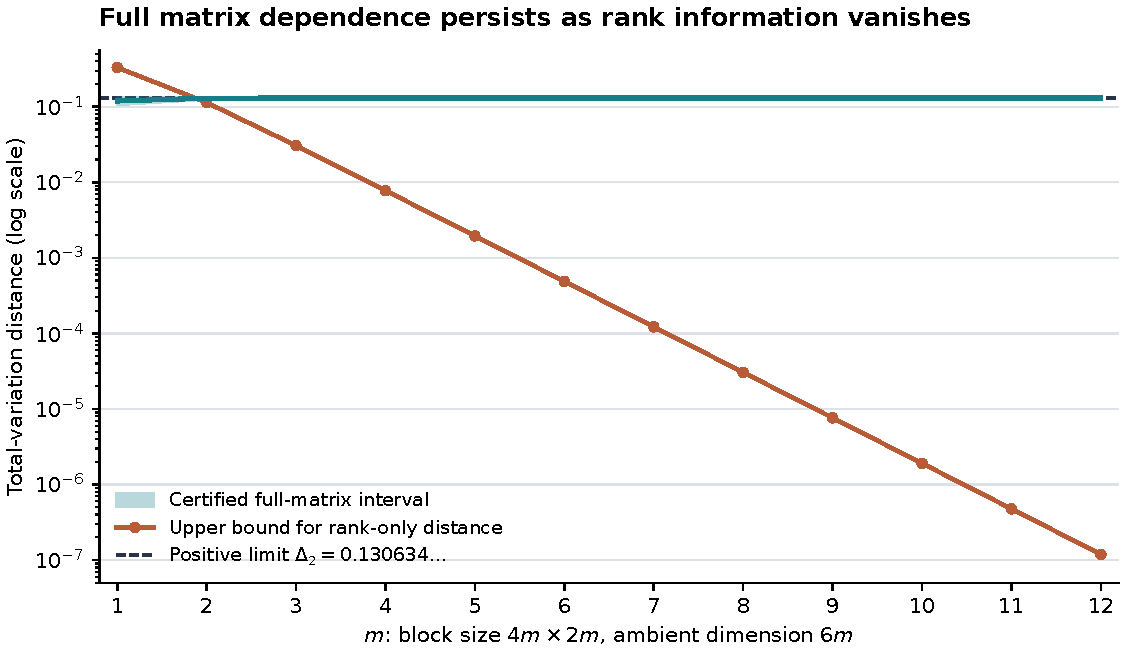
\includegraphics[width=0.96\linewidth]{figures/boundary_bounds.pdf}
\caption{The sequence $q=2$, $a=4m$, $b=2m$, $2N=6m$. The shaded band is the rigorous full-matrix enclosure \eqref{eq:finiteenclosure}; the decreasing curve is the rank-only upper bound \eqref{eq:rankbound}. The horizontal line is $\Delta_2$. These are analytic bounds, not simulation estimates.}
\label{fig:bounds}
\end{figure}

\section{Verification, reproducibility and limits}
\label{sec:checks}

\subsection{Independent finite enumeration}
The proof is not based on numerical evidence. To detect algebraic, normalizing and characteristic-two errors, a separate program enumerates actual injective frames, records their cross Gram matrices and intersection dimensions, and compares the exact counts with Theorem~\ref{thm:law}. Its field implementation for $\F_4$ uses the genuine extension $\F_2[x]/(x^2+x+1)$.

The completed run checked $329\,957$ frame-pair observations, $35\,230$ matrix outcomes and $130\,773$ joint matrix/intersection outcomes, including $16\,777$ zero-probability matrix outcomes. It covers every realizable alternating source and target form in the following small configurations, along with the indicated nonsingular cases:
\begin{center}\small
\begin{tabular}{ccl}
\toprule
Field & Ambient dimension & Block dimensions $(a,b)$\\
\midrule
$\F_2$ & 2 & $(1,1)$\\
$\F_3$ & 2 & $(1,1)$\\
$\F_2$ & 4 & $(2,2),(3,2),(3,3)$\\
$\F_3$ & 4 & $(2,2)$\\
$\F_4$ & 4 & $(2,2)$\\
$\F_2$ & 6, 8 & $(4,2),(6,2)$, nonsingular restricted forms\\
\bottomrule
\end{tabular}
\end{center}
All comparisons passed. The checks include the exact support test, conditional intersection law, boundary likelihood signs and optimal-test total variation identity. For example, at $q=2$, $(a,b)=(6,2)$ in ambient dimension eight, the full distance is $273/2176$, while the rank distance is $399/34816$. Exact machine-readable output is supplied.

\subsection{Contents and commands}
\begin{itemize}[leftmargin=1.5em]
\item \code{report.tex} and \code{report.pdf}: this self-contained note.
\item \code{code/compression_law.py}: integer and rational evaluators for the formulas, support, conditional intersections, first correction and certified constants.
\item \code{code/verify_exhaustive.py}: independent enumeration of actual frames, including extension-field arithmetic.
\item \code{code/reproduce.py}: numerical enclosures, the figure, and additional formula checks.
\item \code{results/}: exact verification output, certified constants and finite bounds.
\item \code{source_audit.md}, \code{literature_review.md}, \code{sources.json}: precise source and priority information.
\item \code{formalization_plan.md}: a dependency-oriented route to formalization, without claiming a completed Lean proof.
\end{itemize}
The core counting and exhaustive verifier use Python's standard library. Reproducing the figure requires Matplotlib. From the archive directory run
\begin{verbatim}
python3 code/verify_exhaustive.py
python3 code/reproduce.py
pdflatex -halt-on-error report.tex
pdflatex -halt-on-error report.tex
\end{verbatim}
The scripts write their results under \code{results/}. The mathematical statements are valid for every prime-power $q$; the exhaustive experiments cover only the explicitly listed finite fields and dimensions.

\subsection{What has and has not been established}
The note supplies complete proofs of the arbitrary-compression law, exact support and minimal-completion theorem, sharp fixed-dimension rate, and nondegenerate rectangular boundary theorem. These results answer a concrete question in the supplied article and provide quantitative consequences not stated there. The new work has not been formalized in Lean or subjected to external peer review. The finite checks are supplementary validation, not a proof assistant's kernel certificate.

The literature search identifies substantial classical antecedents. A publication-level priority claim would require a more exhaustive comparison, especially of the older form-representation papers in full. Nothing here proves a further RH, Artin holomorphy, or an arithmetic nonvanishing result. The gain is a complete and usable theorem in the matrix-statistics branch of the source program, with a precise explanation of when rank diagnostics fail.

\clearpage
\begin{thebibliography}{9}
\raggedright
\bibitem{upstream}
\texttt{lsernau/grh-lean}, \emph{GRH for Dirichlet $L$-functions, in Lean 4}, commit \sourcecommit. Main statements, guide and selected reduction files, inspected November 26, 2026 (Pacific).
\url{https://github.com/lsernau/grh-lean}.

\bibitem{article}
Vladimir Reshetnikov, ProveIt repository, \emph{Beyond the Riemann hypothesis for Dirichlet $L$-functions: consequences, transfers and limits}, merged article, commit \articlecommit. In particular \code{Article/sections/spn.tex}, question \code{spn:q:symplectic}.
\url{https://github.com/VladimirReshetnikov/ProveIt/tree/main/Analysis/GeneralizedRiemannHypothesis/Article}.

\bibitem{wan}
Zhe-Xian Wan, \emph{Representations of Forms by Forms in a Finite Field}, Finite Fields and Their Applications \textbf{1} (1995), 297--325.
\url{https://doi.org/10.1006/ffta.1995.1024}.

\bibitem{weizhang}
Hongzeng Wei and Yibin Zhang, \emph{The number of solutions to the alternate matrix equation over a finite field and a $q$-identity}, Journal of Statistical Planning and Inference \textbf{94} (2001), 349--358.
\url{https://doi.org/10.1016/S0378-3758(00)00265-2}.

\bibitem{guo}
Jun Guo, Fenggao Li and Kaishun Wang, \emph{Anzahl formulas of subspaces in symplectic spaces and their applications}, Linear Algebra and its Applications \textbf{438} (2013), 3321--3335.
\url{https://doi.org/10.1016/j.laa.2012.12.008}.

\bibitem{deboeck}
Maarten De Boeck and Geertrui Van de Voorde, \emph{Anzahl theorems for trivially intersecting subspaces generating a non-singular subspace I: symplectic and hermitian forms}, Linear Algebra and its Applications \textbf{699} (2024), 367--402.
\url{https://doi.org/10.1016/j.laa.2024.07.004}; \url{https://arxiv.org/abs/2407.07486}.
\end{thebibliography}
\end{document}
